\chapter{NoSQL- Datenbanken}
NoSQL- Datenbanken machen heutzutage ein Revolution.
\section{MongoDB}
siehe\cite{Hollosi.2012}, siehe \cite{LloretIvorra.2013} Von Geodaten bis NoSQL: Leistungsstarke PHP-Anwendungen \url{http://ezproxy.bib.fh-muenchen.de:2125/doi/book/10.3139/9783446431225}\newline
Dokumentdatenbanken gruppieren die Daten in einem strukturierten Dokument, typischerweise in einer JSON-Datenstruktur. Auch MongoDB verfolgt diesen Ansatz und bietet darauf aufbauend eine reichhaltige Abfragesprache und Indexe auf einzelne Datenfelder. Die Möglichkeiten der Replikation und des Shardings zur stufenlosen und unkomplizierten Skalierung der Daten und Zugriffe macht MongoDB auch für stark frequentierte Websites äußerst interessant.
\newline
\newline
MongoDB bietet zudem auch Map/Reduce zur Datenverarbeitung an. Map/Reduce ist ein Kernbaustein zur Verarbeitung großer Datenmengen (auch in anderen NoSQL-Datenbanken), da mit diesem Ansatz die Berechnungen auf einfachem Wege auf viele Server zur parallelen Berechnung verteilt werden können. Mehr dazu erfahren Sie in Abschnitt 14.6. Siehe auch weitere Kapitel wie 14.2 Datenbanken und Datenschema


Die nicht-relationale Datenbank 'MongoDB' macht mit einem effizienten Dokument-orientierten Ansatz, einfacher Skalierbarkeit und hoher Flexibilität dem bewährten MySQL-System zunehmend Konkurrenz. Der Begriff NoSQL steht, anders als zunächst von den meisten erwartet, nicht für "kein SQL", sondern für "nicht nur SQL" (Not only SQL). Ziel des neuen Ansatzes ist es vielmehr, relationale Datenbanken sinnvoll zu ergänzen wo sie Defizite aufzeigen. Entstanden ist dieses Konzept in erster Linie als Antwort zur Unflexibilität, sowie zur relativ schwierigen Skalierbarkeit von klassischen Datenbanksystemen, bei denen die Daten nach einem stark strukturierten Modell gespeichert werden müssen.\footnote{NoSQL: \url{http://www.computerwoche.de/a/datenbanksysteme-fuer-web-anwendungen-im-vergleich,2496589}} \newline\newline
In Zeiten von Web 2.0, Cloud Computing und sozialen Netzen wachsen die Datenmengen bei Web-Anwendungen dramatisch. Damit steigen die Anforderungen an Datendurchsatz und Skalierbarkeit der darunter liegenden Datenbanken immer weiter an. Ein Paradebeispiel für diese Problematik ist Twitter. Wie der US-Blog "TechCrunch" im Juni 2011 berichtete, muss die IT-Landschaft des populären Informationsnetzes mittlerweile rund 200 Millionen Tweets am Tag bewältigen. Ein Jahr zuvor waren es "nur" 65 Millionen. Bei solchen datenintensiven Applikationen leiden relationale Datenbanken üblicherweise unter Leistungsproblemen und stoßen oft an ihre Grenzen. Aus diesem Grund setzt Twitter neben MySQL mittlerweile auch auf NoSQLLösungen, um die Verfügbarkeit und Performance seines Dienstes zu verbessern.\newline\newline
Das System 'MongoDB' wurde 2009 vom amerikanischen Startup 10gen nach rund zwei Jahren Entwicklung der Öffentlichkeit als Open-Source-Lösung vorgestellt. Der etwas gewöhnungsbedürftige Name stammt von dem englischen Begriff "humongous", der sich ins Deutsche mit 'gigantisch'  beziehungsweise "riesig" übersetzen lässt. Die Lösung basiert auf der Programmiersprache C++ und ist für die Betriebssysteme Windows, Mac OS X und Linux erhältlich. Sowohl 32-Bit- als auch 64-Bit-Systeme werden unterstützt.\newline\newline
Wie der Hersteller erklärt, ist die Lösung auf starke Leis-tung, große Datenmengen, hohe Flexibilität sowie einfache Skalierbarkeit ausgelegt.
\section{Tabellen haben ausgedient - Dokumente als Datensätze}
Die nichtrelationale Datenbank MongoDB speichert Datensätze in Form von Dokumenten im JSON-Format. Diese sind Javascript-Objekten sehr ähnlich. Der entscheidende Unterschied zu MySQL besteht darin, dass MongoDB dokumentenorientiert arbeitet. Dokumentenbasierende Datenbanken sind auf eine schemafreie Struktur ausgelegt. Bei MongoDB gibt es also kein festes Tabellenschema und dadurch beispielsweise auch keine zwingenden Relationstabellen und "Joins", die mit der Weiterentwicklung und dem Ausbau der Datenbank immer komplexer werden. Stattdessen lassen sich Relationen entweder direkt im Datensatz speichern oder bei Bedarf individuell bei der Datenabfrage erstellen. Dadurch ist die Datenstruktur wesentlich flexibler als bei MySQL und lässt sich einfach horizontal skalieren.\newline\newline
Statt von Tabellen spricht man bei MongoDB von Kollektionen (Collections). Jede Kollektion kann Dokumente beinhalten analog zu Zeilen beziehungsweise Datensätzen in einer MySQL-Tabelle. Dokumente werden im so genannten BSON-Format gespeichert und ausgegeben. Sie sind dann Javascript-Objekten sehr ähnlich. Das Format stammt von dem kompakten JSON-Format (Javascript Object Notation) ab und ist, wie das Präfix "Binary" (Binary JSON = BSON) andeutet, für eine Overhead-arme Darstellung von binären Datenobjekten ausgelegt. Jedes Dokument kann dabei eine beliebige Anzahl an Feldern besitzen, während eine verschachtelte Array-Struktur ebenfalls möglich ist. Zudem dürfen Dokumente auch innerhalb eines Dokuments gespeichert werden.



\section{Introduction}
Siehe in Deutsch: \url{https://www.iks-gmbh.com/assets/downloads/Einfuehrung-in-MongoDB-iks.pdf}\newline
\section{CRUD}
\section{Schema Design}
\section{Performance}
Siehe in Deutsch über Indexes: \url{https://books.google.de/books?id=kRUbDAAAQBAJ&pg=PA53&lpg=PA53&dq=index+in+mongodb+was+ist+da&source=bl&ots=80Kgw664kZ&sig=rEhHo3g4JRVAVXwUr_In5xzWB8c&hl=en&sa=X&ved=0ahUKEwiBvd_VsbfQAhVDtBQKHX4_ASAQ6AEINjAC#v=onepage&q=index%20in%20mongodb%20was%20ist%20da&f=false}\newline

\section{Aggregation Framework}
\section{Application Engineering}

\section{Sharding}
MongoDB bietet mit AutoSharding ein Feature, das es ermöglicht, einen Datenbankserver automatisch auf verschiedene physikalische Maschinen aufzuteilen und somit die Datenbank horizontal zu skalieren. Um das Sharding bei MongoDB zu konfigurieren, werden drei Komponenten benötigt...., siehe Sharding \url{https://www.iks-gmbh.com/assets/downloads/Einfuehrung-in-MongoDB-iks.pdf
}



\section{ODMs für MongoDB}

ODM ist Object-Document Mapper für nichtrelationale Datenbanken wie MongoDB, Apache Cassandra etc.

\subsection{Morphia}
Morphia is the Java Object Document Mapper for MongoDB \url{http://mongodb.github.io/morphia/}

\subsection{Doctrine}
The Doctrine MongoDB ODM project is a library that provides a PHP object mapping functionality for MongoDB. \url{https://github.com/doctrine/mongodb-odm}

\section{Beziehungen}
Folgenden Relationen wie One-to-One \textbf{Teilabschnitt \ref{1:1}}, One-to-Many \textbf{Teilabschnitt \ref{1:n}} und Many-to-Many \textbf{Teilabschnitt \ref{n:m}} blabla

\subsection{One-to-One}\label{1:1}
bla

\subsection{One-to-Many}\label{1:n}
bla

\subsection{Many-to-Many}\label{n:m}
bla

\section{Storage Engines}

\subsection{MMAPv1}
MMAPv1 is default a storage engine.
MMAPv1 automatically allocates power-of-two-sized documents when new documents are inserted
This is handled by the storage engine.
MMAPv1 is built on top of the mmap system call that maps files into memory
This is the basic idea behind why we call it MMAPv1.

\subsection{WiredTiger}
To invoke a WiredTiger storage engine, you would use:

\begin{listingsbox}[label={lst:X}]{myshell}{Something else}
> killall mongod
\end{listingsbox}
\begin{listingsbox}[label={lst:X}]{myshell}{Something else}
> mkdir WT
\end{listingsbox}

\begin{listingsbox}[label={lst:X}]{myshell}{Something else}
> mongod -dbpath WT --storageEngine wiredTiger
\end{listingsbox}

Dann mongo starten mit 'mongo', dann:

\begin{listingsbox}[label={lst:X}]{myshell}{Something else}
> db.foo.insert({'name':'andrew'})
\end{listingsbox}

\begin{listingsbox}[label={lst:X}]{myshell}{Something else}
> db.foo.stats()
\end{listingsbox}

 -> man bekommt die Information über die Collection.
Which of the following are features of the WiredTiger storage engine?\newline
- Document-level concurrency\newline
- Compression

\section{Indizes}
Index hilft, Datenbanken zu optimieren. Die nachfolgende \autoref{img:index1} demonstriert

\begin{figure}[H]
	\centering
	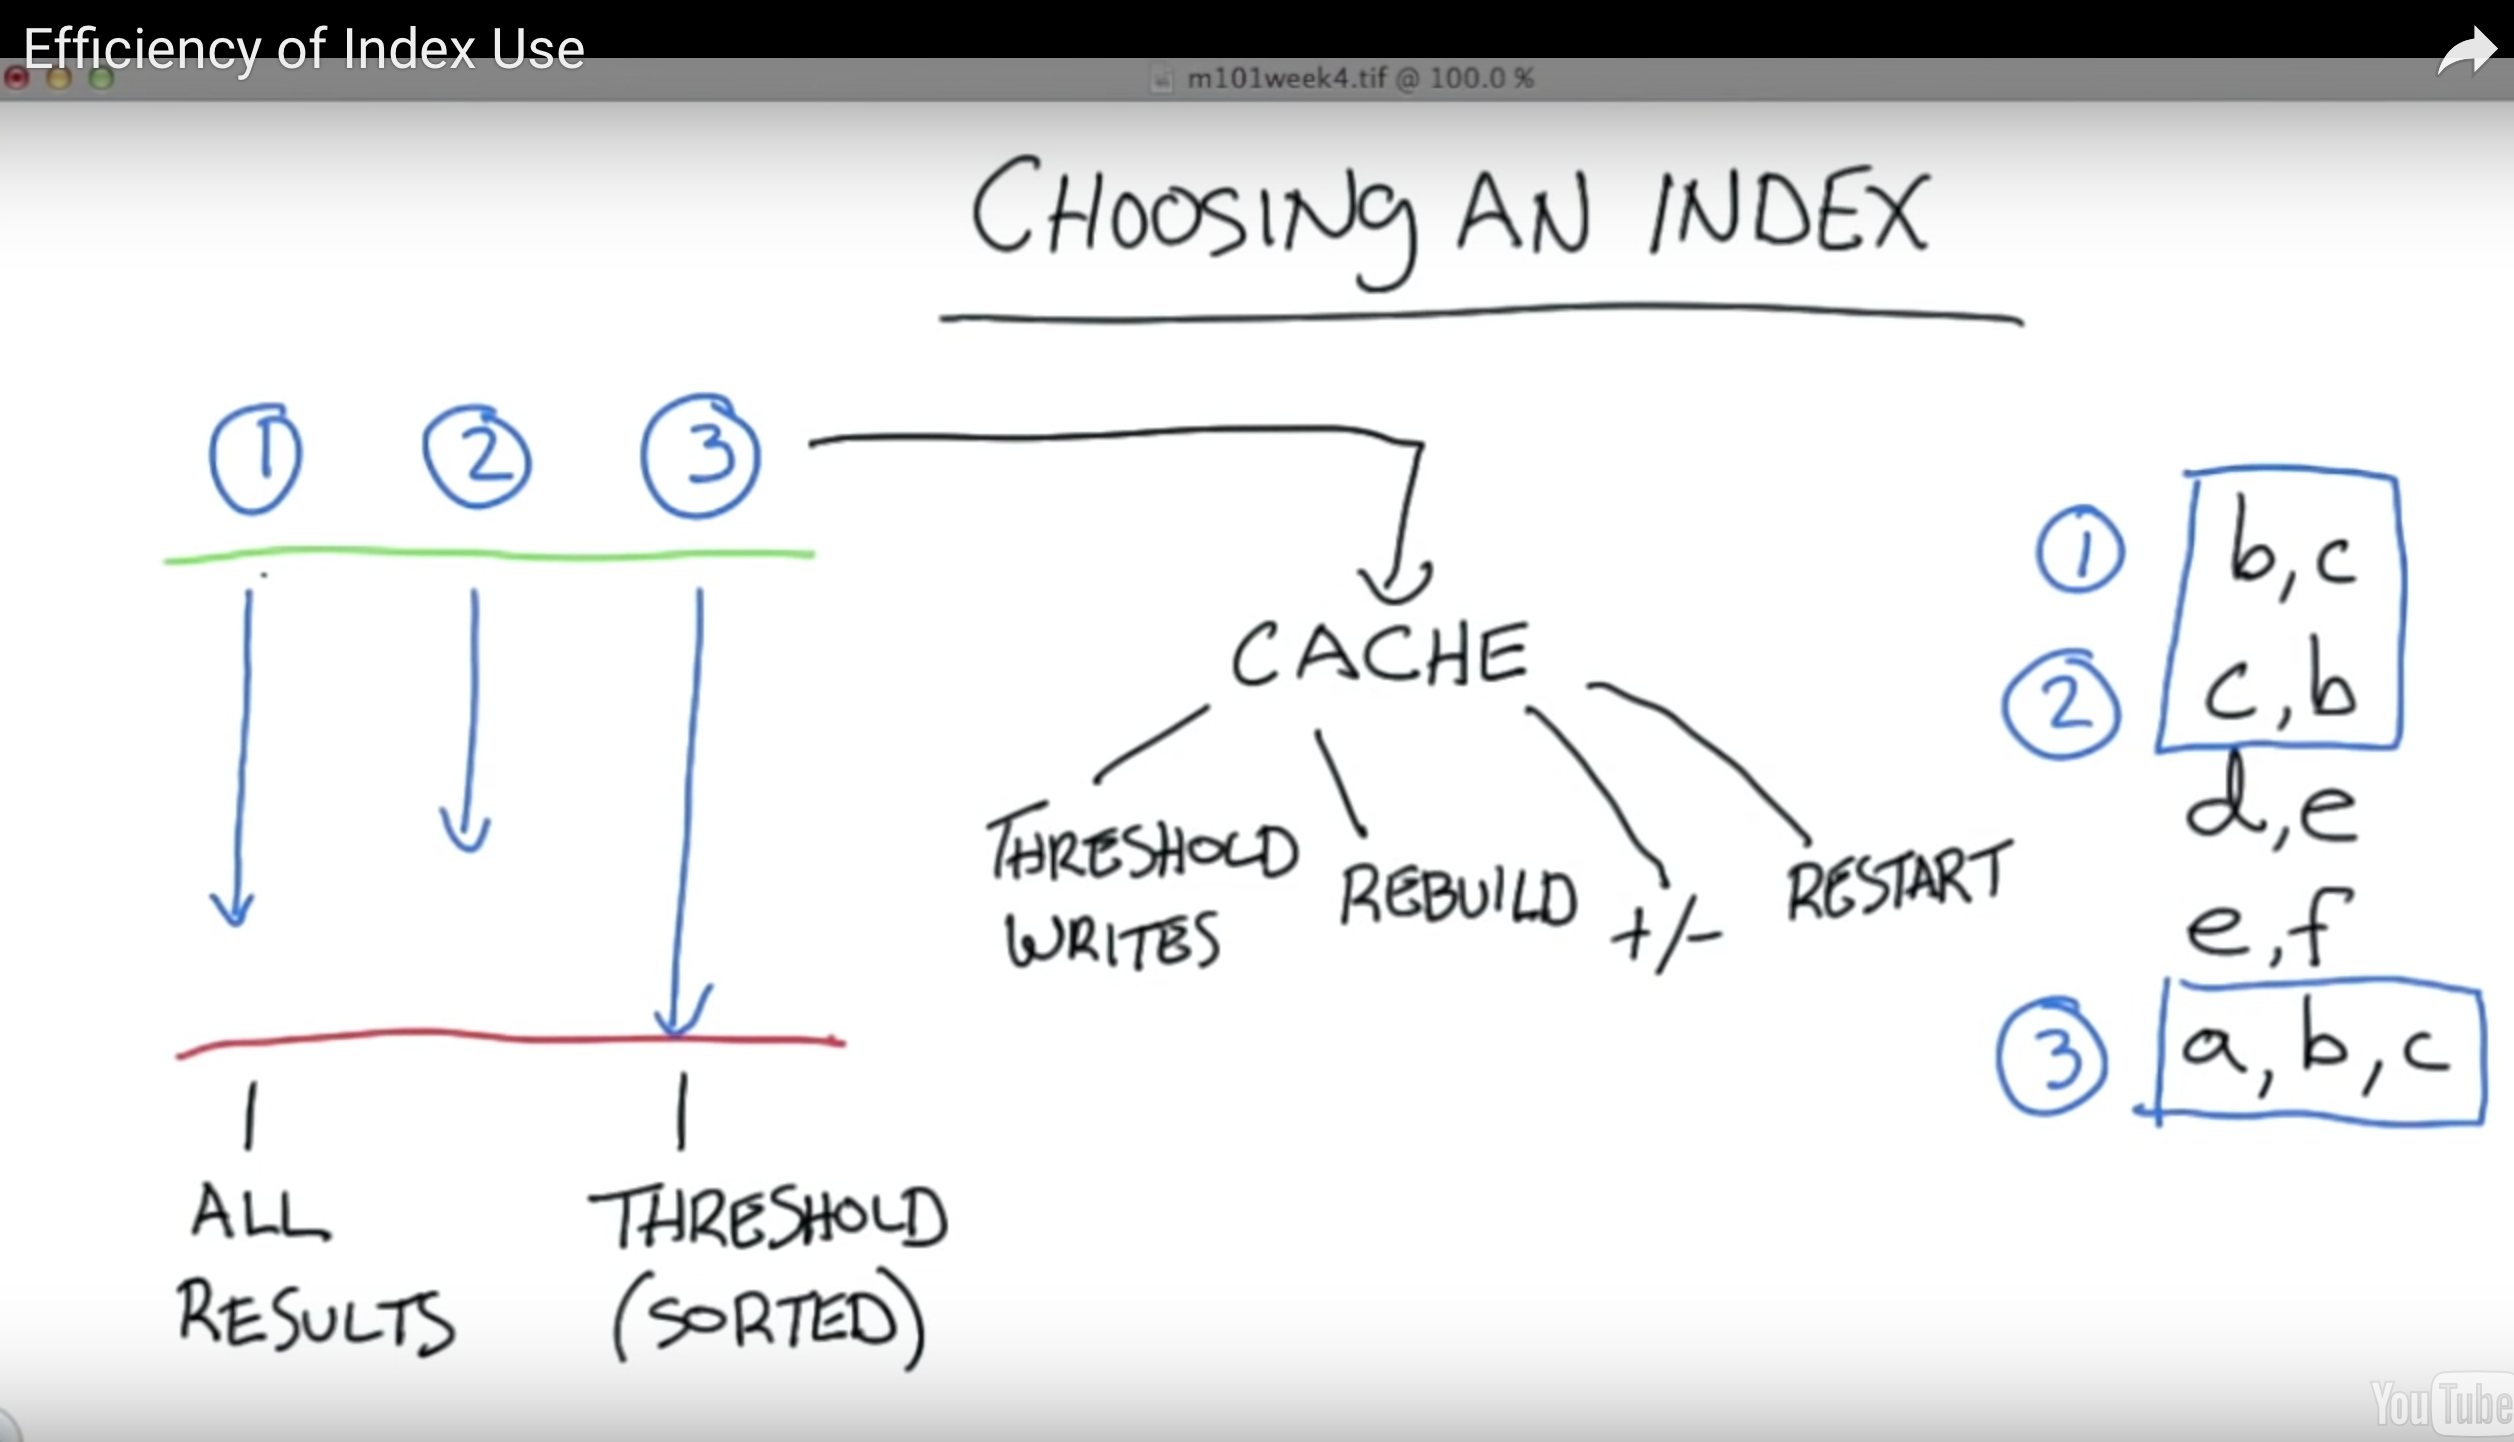
\includegraphics[width=0.7\textwidth]{resources/efficiencyOfIndexUse}
	\caption{Efficiency of Index Use}
	\label{img:index1}
\end{figure}

\url{https://docs.mongodb.com/manual/indexes/}
Neben dem obligatorischen Primär-Index auf dem Feld \_id, das in jedem Dokument existieren und pro Collection eindeutig sein muss, können Sie in MongoDB bis zu 63 weitere Sekundär-Indizes pro Collection anlegen, um Suchanfragen zu beschleunigen. Ein Sekundär-Index kann auf einem einzelnen Feld oder einer Gruppe von Feldern angelegt werden.%\footnote{Indizes: \url{https://www.informatik-aktuell.de/betrieb/datenbanken/mongodb-fuer-software-entwickler.html}}

Which optimization will typically have the greatest impact on the performance of a database?\newline
Adding appropriate indexes on large collections so that only a small percentage of queries need to scan the collection.

\subsection{Creating Indexes}
blabla

\begin{listingsbox}[label={lst:X}]{myshell}{Something else}
> db.students.createIndex();
\end{listingsbox}

blabla

\begin{listingsbox}[label={lst:X}]{myshell}{Something else}
> db.students.explain().find();
\end{listingsbox}

Quiz: Please provide the mongo shell command to add an index to a collection named students, having the index key be class, student\_name.
Neither will go in the "-1" direction..

\begin{listingsbox}[label={lst:X}]{myshell}{Something else}
> db.students.createIndex({student\_name:1, class:1});
\end{listingsbox}

\begin{listingsbox}[label={lst:X}]{myshell}{Something else}
> db.students.dropIndex({student_name:1});
\end{listingsbox}

\subsubsection{Multikey Indexes}
blabla
\subsubsection{Index Creation Option, Unique}
für jedes attribut kann man Unique definieren, d.h. doppelte Werte dürfen nicht vorkommen\newline\newline

\begin{listingsbox}{myshell}{Something else}
> db.students.createIndex({student_id : test}, {unique:true});
\end{listingsbox}

Please provide the mongo shell command to create a unique index on student\_id, class\_id, ascending for the collection students.

\begin{listingsbox}[label={lst:X}]{myshell}{Something else}
> db.students.createIndex({student_id:1, class_id:1}, {unique:true});
\end{listingsbox}

\subsubsection{Index Creation, Sparse}

Im Fall, wenn ein Attribut nicht in allen Dokumenten vorkommt, aber für dieses ein Unique Index definiert werden soll, muss Folgendes verwendet werden:

\begin{listingsbox}[label={lst:X}]{myshell}{Something else}
> db.students.createIndex({cell:1}, {unique:true, sparse:true});
\end{listingsbox}

blabla, siehe den Shellbefehl, blabla

\begin{listingsbox}[label={lst:X}]{myshell}{Something else}
> db.students.createIndex({student_id:1, class_id:1}, {unique:true});
\end{listingsbox}
siehe Codeauszug 

\section{Prototyp}
Kommentare zu den Fotos hinzufügen, Eingebettete Kommentare, siehe \url{http://ezproxy.bib.fh-muenchen.de:2125/doi/pdf/10.3139/9783446431225.014}

\section{Replikation und Verfügbarkeit}
MongoDB kann Server in Replikationsgruppen anordnen, damit bei Ausfall eines Servers die Verfügbarkeit der Datenbank trotzdem gewährleistet ist. blabla
\section{Aggregation Framework}
How good is it? Mapping between SQL and Aggregation
\section{Fazit}
Siehe Listing \ref{lst:X} \newline 
Doch wie der Begriff Not only SQL (NoSQL) andeutet, stehen beide Datenbanksysteme nicht unbedingt in direkter Konkurrenz zueinander, sondern können sich gegenseitig ergänzen. Dennoch, wenn es um die persistente Datenspeicherung bei Web-Anwendungen geht, stellen relationale Datenbanken nicht mehr die einzige Alternative dar. Bei eigenen Projekten wären Entwickler heute also gut beraten, die Vor- und Nachteile der beiden Systeme gegenüberzustellen und entsprechend den eigenen Anforderungen und Prioritäten zu bewerten. Muss das System mit großen Datenmengen effizient umgehen können? Werden hohe Anforderungen an Skalierbarkeit und Flexibilität der Datenbank gestellt? Sollen sich die Daten über mehrere Server verteilen lassen? Sind häufige Änderungen an der Datenstruktur in Zukunft zu erwarten? Wenn Sie die meisten dieser Fragen mit "Ja" beantworten, dann sollten Sie sich MongoDB zumindest näher anschauen.\newline\newline

Daten in MongoDB verfügen über ein flexibles Schema. Kollektionen (=Collections) erzwingt keine Struktur.

\begin{listingsbox}[label={lst:conn}]{myJava}{Verbindungsaufbau}
public static void main(String[] args) {

	MongoClient mongoClient = new MongoClient("localhost", 27017);
        MongoDatabase db = mongoClient.getDatabase("test");
        MongoCollection<Document> collectionOfZips = db.getCollection("zips");
        
        // weitere CRUD-Operationen mit der ausgewählten Kollektion
}
\end{listingsbox}
Test \ref{lst:conn}
\section{Apache Cassandra}